%% This classfile tries to implement the lay-out of the beamer style beamerthemekuleuven2. This .sty-file can be downloaded here: https://www.kuleuven.be/communicatie/marketing/templates/presentatiemateriaal/index.html Not all options of the style are implemented in this class, for its purpose is merely to mimic the lay-out, and to provide a way to change the lay-out of presentations that were made using the "old" kulakbeamer class. For new documents, we recommend using the .sty-file instead.

\documentclass
   [kulak] % options: kul or kulak (default), handout 
   {kulakbeamer}

\usepackage[dutch]{babel}
\usepackage[utf8]{inputenc}
\usepackage[T1]{fontenc}
\usepackage{textcomp}
\usepackage{siunitx}
\usepackage{subcaption}

\title[HPE]{Human Pose Estimation met OpenPose:}
\subtitle{een toepassing}
\author[Korte naam]{Mathieu Vanooteghem, Isaac Venus \\ 
	en Stan Vanhecke} 
\institute[Kulak]{KU Leuven Kulak}
\date{Academiejaar 2020 -- 2021}

%% Overview at begin of each section; delete if unwanted.

\AtBeginSection[]{
	\begin{frame}
	\frametitle{Overzicht} %Change to "Outline" for English presentation
	{
		\hypersetup{hidelinks} %disable link colors
		\hfill	{\large\parbox{.95\textwidth}{\tableofcontents[currentsection,hideothersubsections]}}
	}
\end{frame}}

\begin{document}

\begin{titleframe}
\titlepage
\end{titleframe}

\begin{outlineframe}[Overzicht]
\tableofcontents
\end{outlineframe}

 % % % Here you go  % % % 

\section{Inleiding}

\begin{frame}
\frametitle{Inleiding}
	\begin{itemize}
		\item stevig prijskaartje aan medische apparatuur
		\item werken met alledaagse technologie
		\item HPE: schatten van lichaamspositie
		\item verschillende toepassingen
	\end{itemize}
\end{frame}



\section[Korte titel]{Theoretische achtergrond}
\begin{frame}
	\frametitle{HPE vergelijken met motion capture}
	\begin{figure}
		\begin{minipage}[b]{.4\linewidth}
			\centering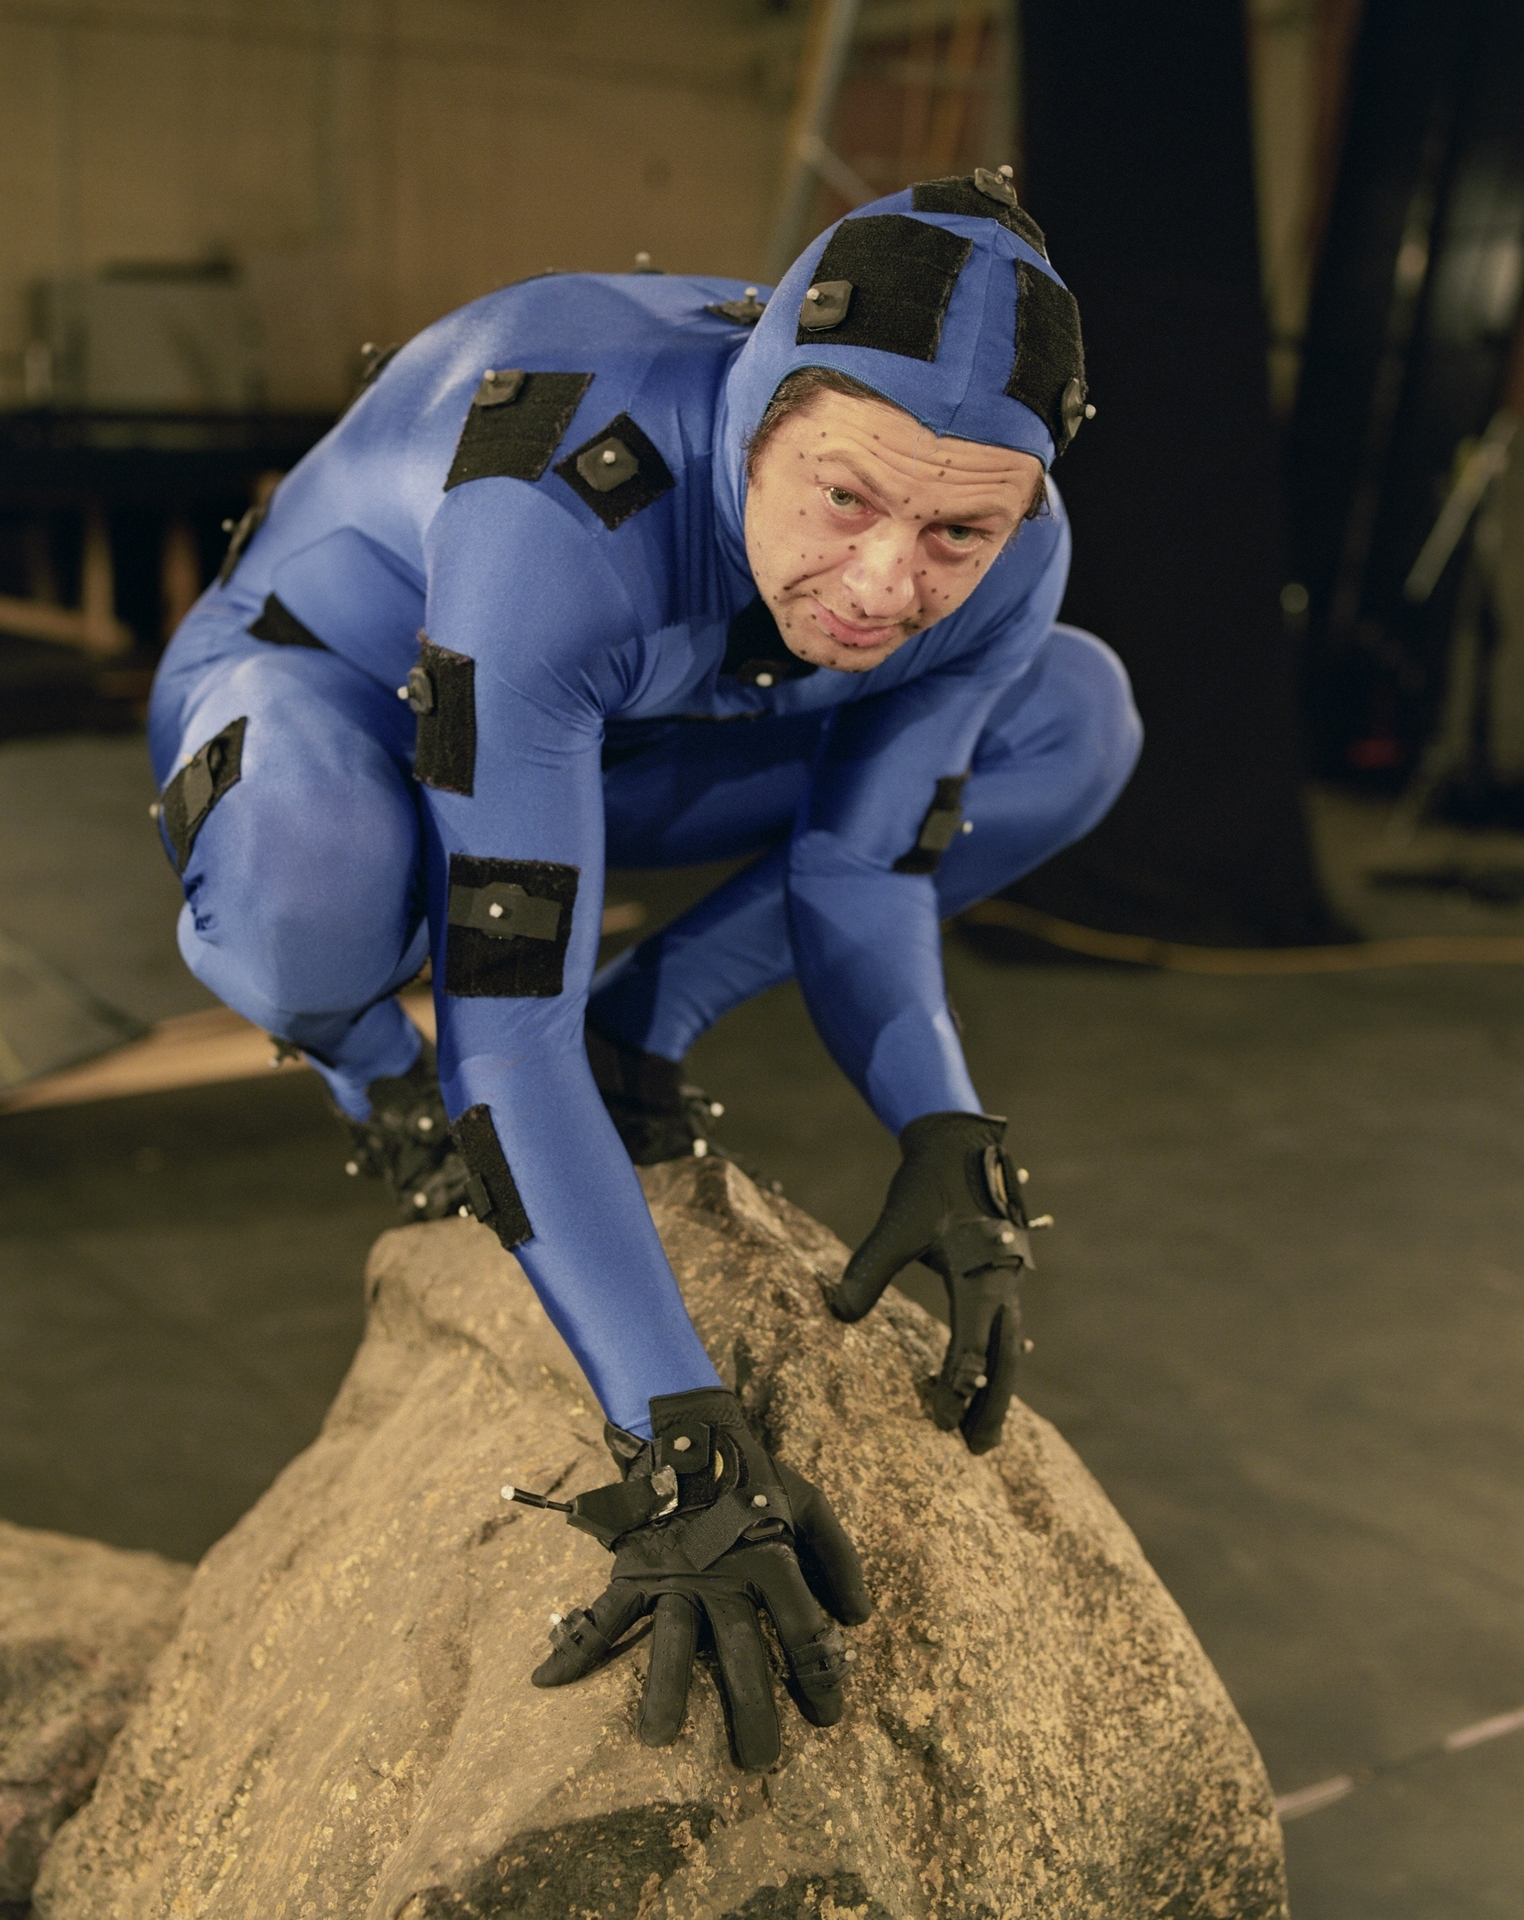
\includegraphics[width= \textwidth]{3D_motion_capture}
			\subcaption{Motion capture pak}\label{fig:1a}
		\end{minipage}%
		\begin{minipage}[b]{.4\linewidth}
			\centering%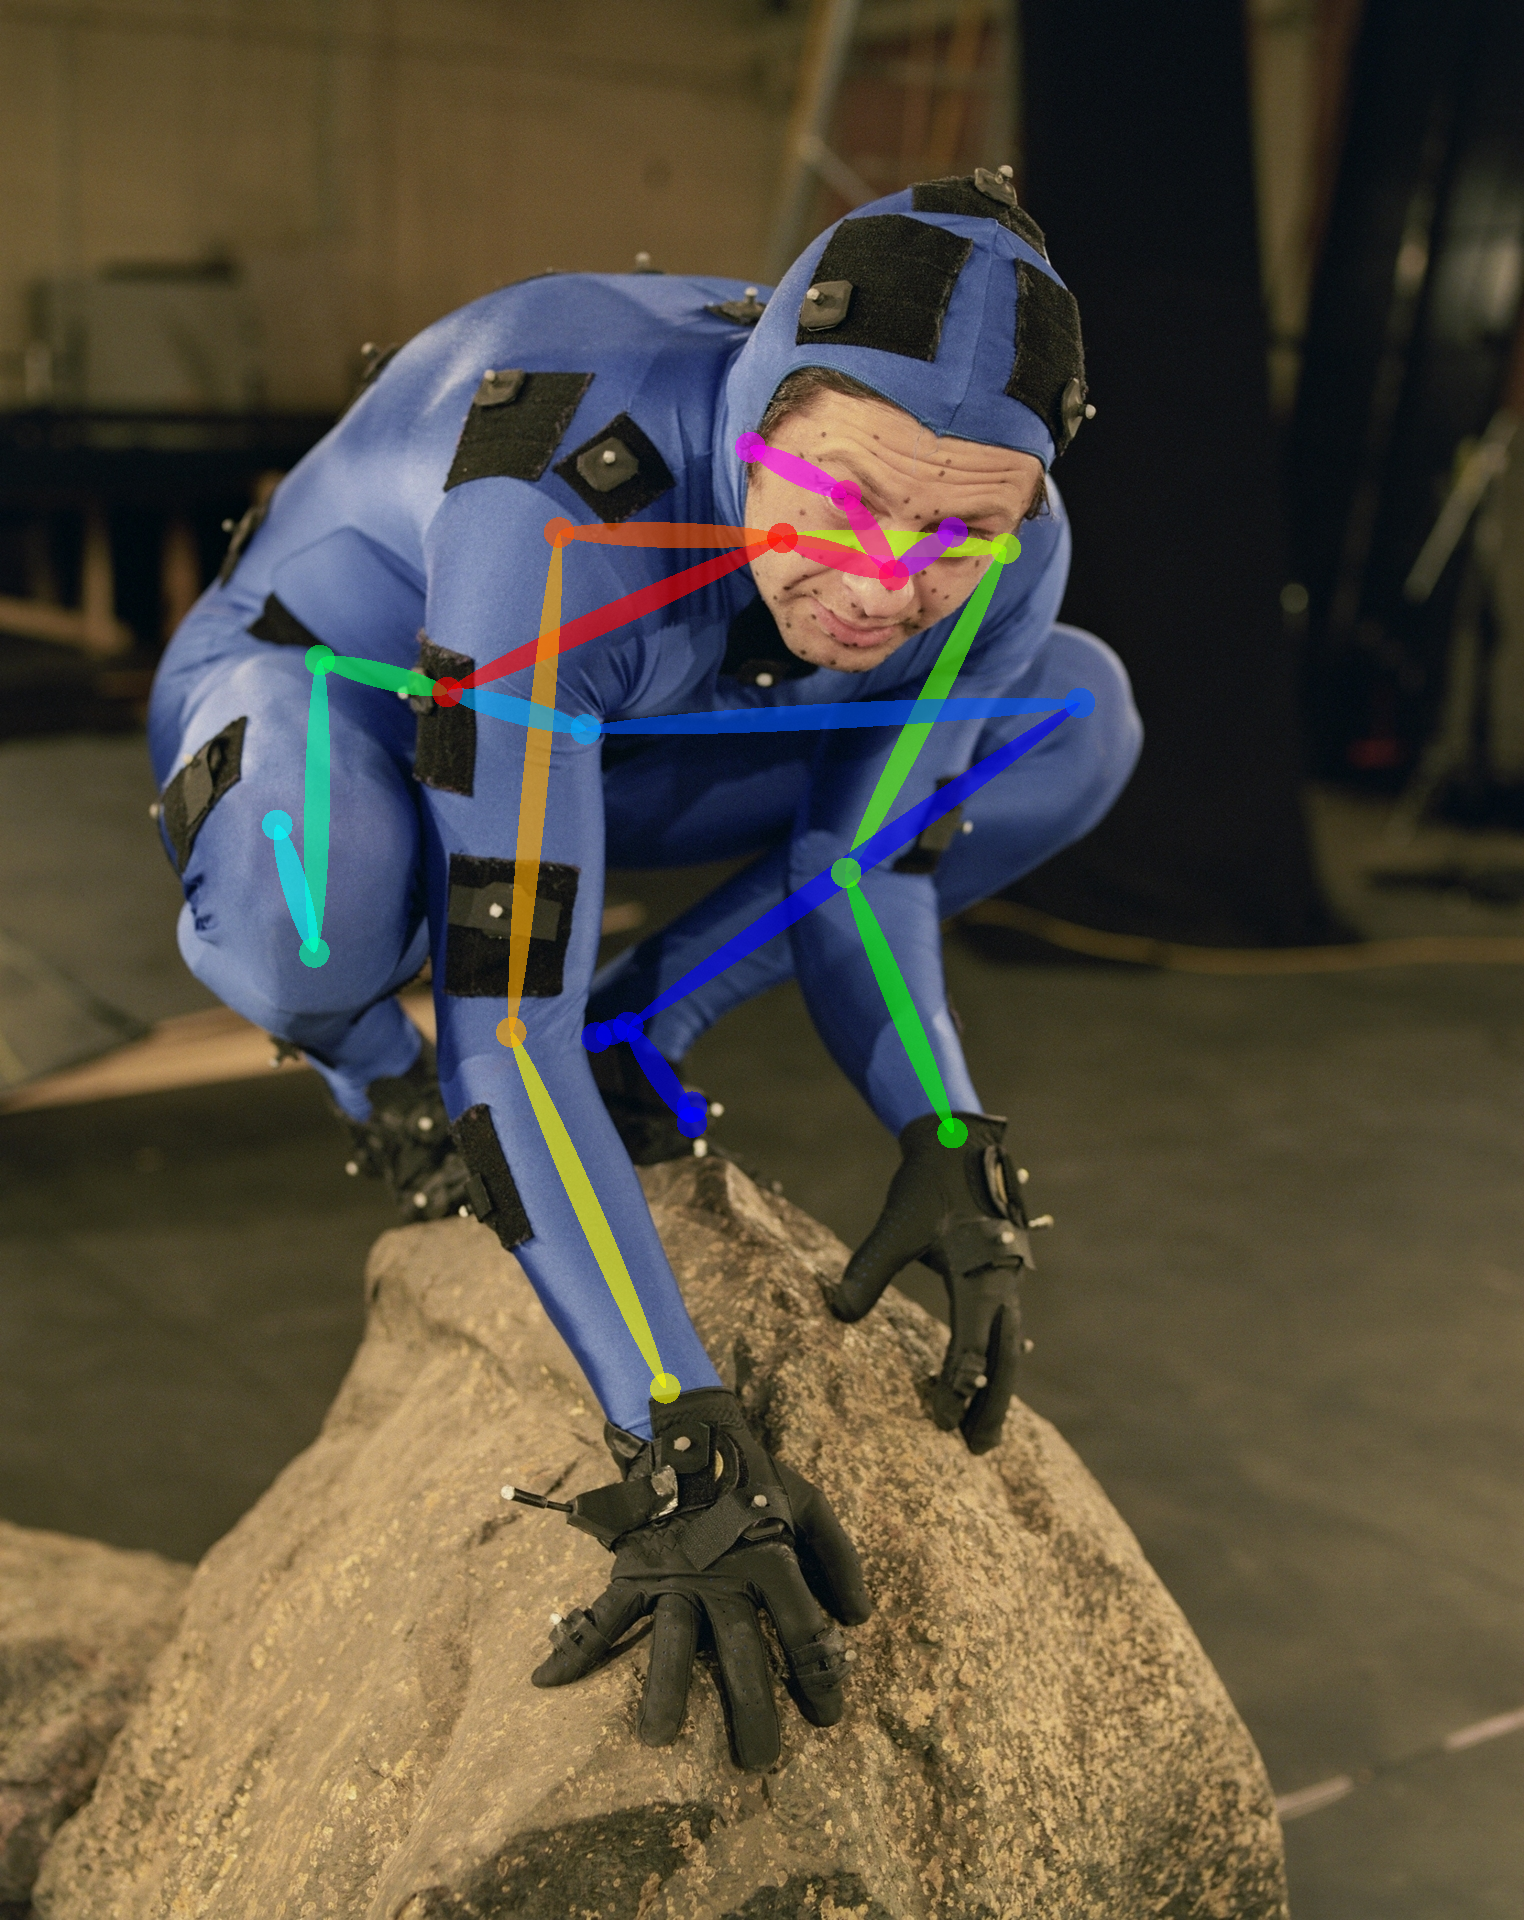
\includegraphics[width= \textwidth]{motion_capture_openpose}
			\subcaption{Schatting van OpenPose}\label{fig:1b}
		\end{minipage}
		%\caption{A figure}\label{fig:1}
	\end{figure}
\end{frame}
\begin{frame}
	\frametitle{HPE vergelijken met motion capture}
	\begin{figure}
		\begin{minipage}[b]{.4\linewidth}
			\centering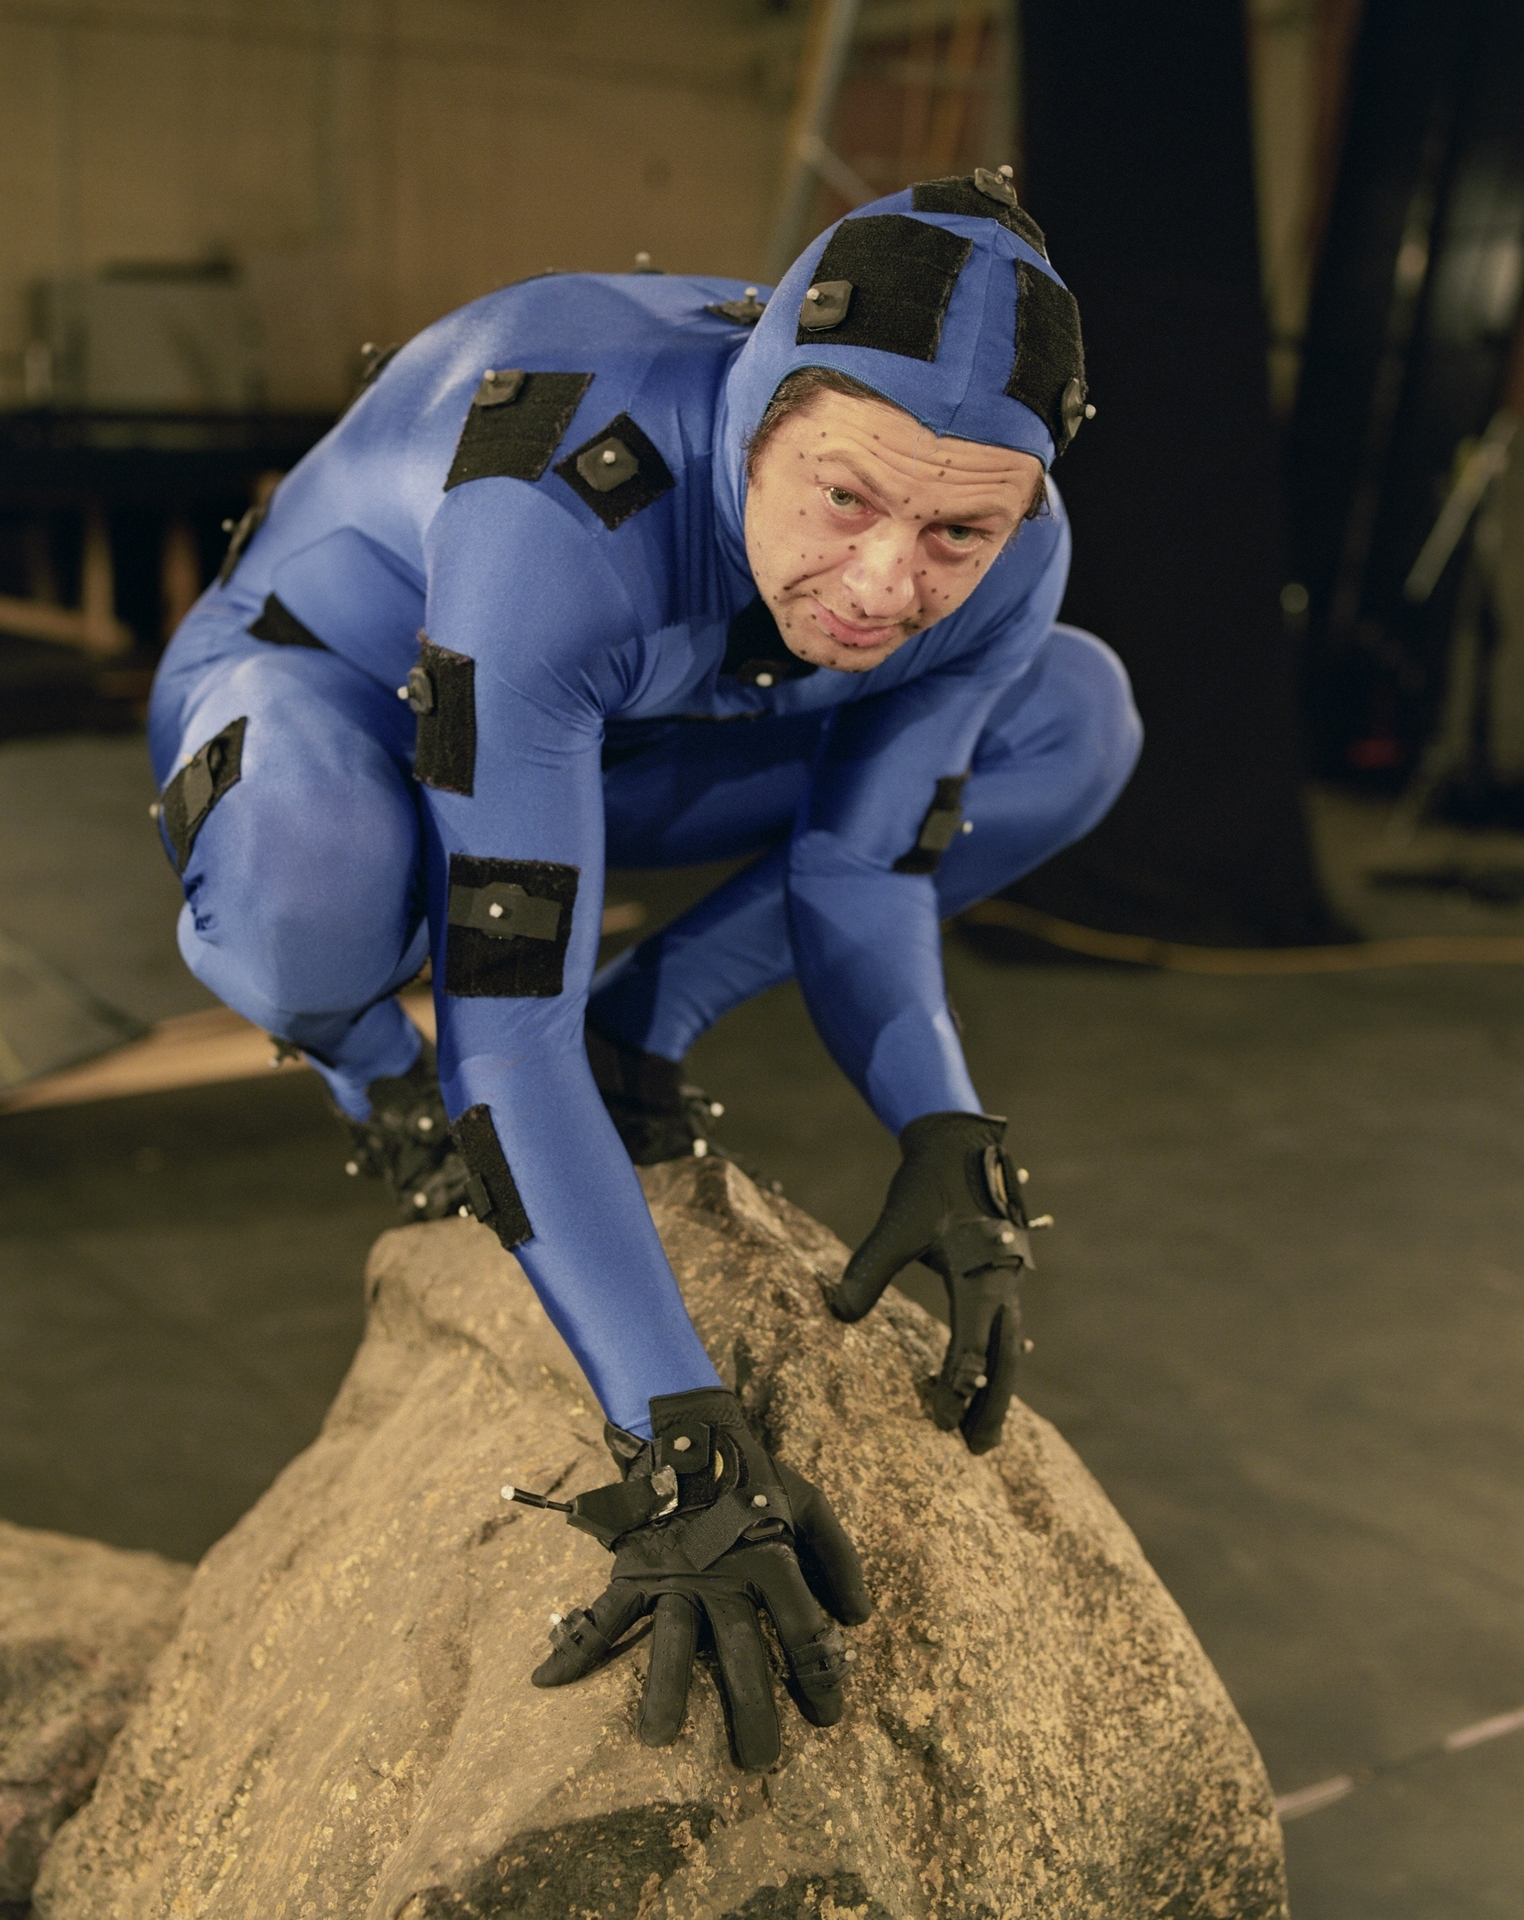
\includegraphics[width= \textwidth]{3D_motion_capture}
			\subcaption{Motion capture pak}\label{fig:1a}
		\end{minipage}%
		\begin{minipage}[b]{.4\linewidth}
			\centering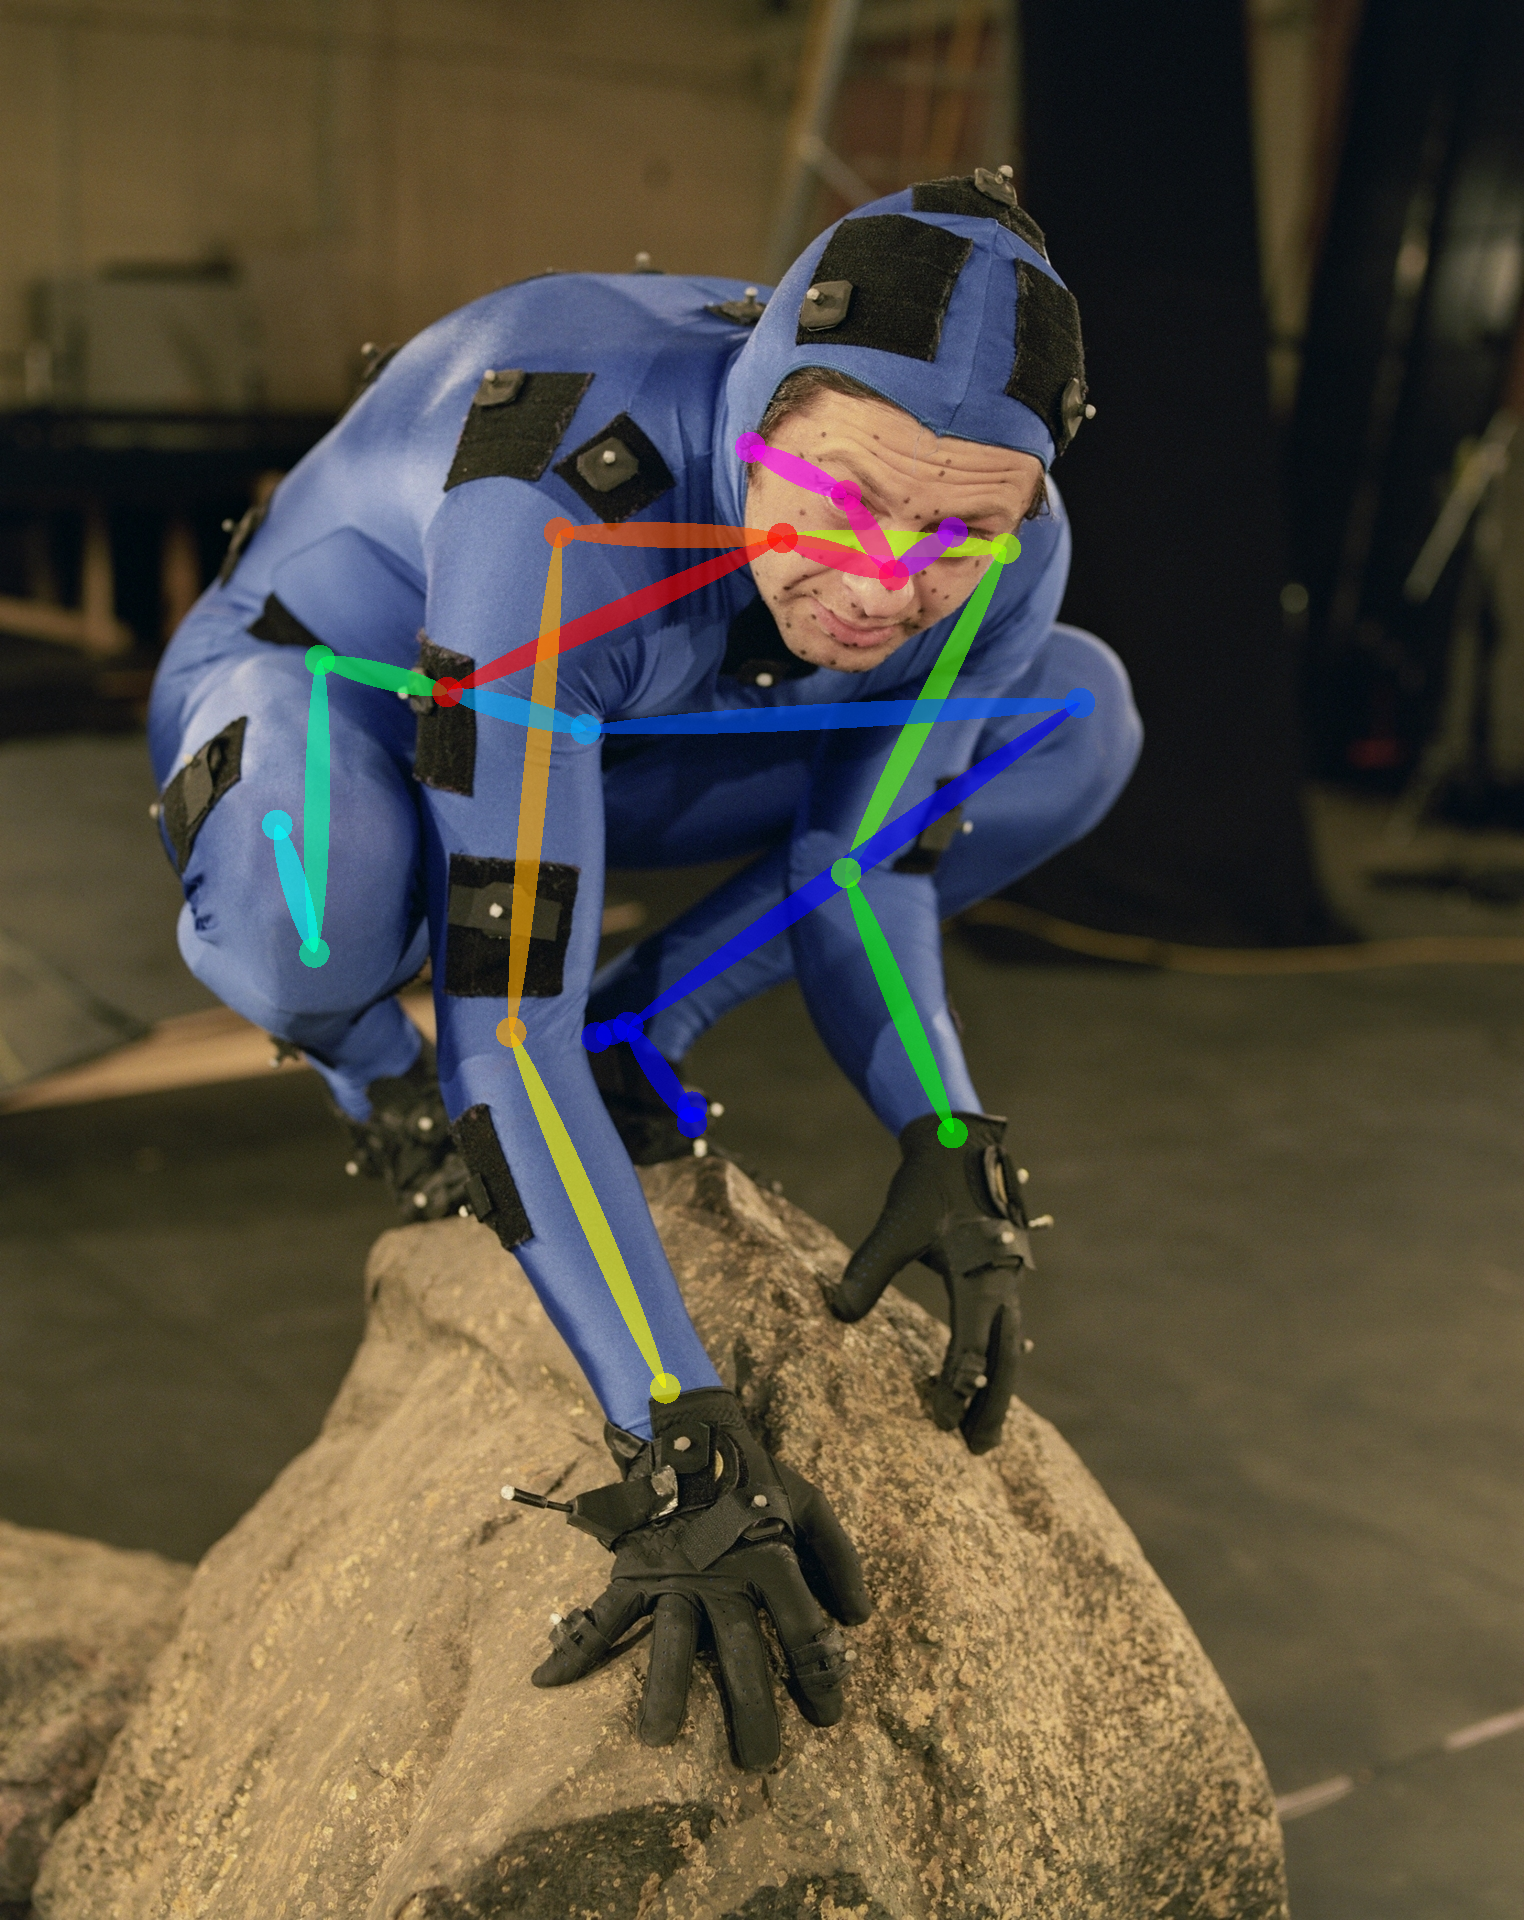
\includegraphics[width= \textwidth]{motion_capture_openpose}
			\subcaption{Schatting van OpenPose}\label{fig:1b}
		\end{minipage}
		%\caption{A figure}\label{fig:1}
	\end{figure}
\end{frame}

\begin{frame}
\frametitle{HPE vergelijken met motion capture}
\begin{center}
	\begin{tabular}{l|l} 
		\textbf{3D motion capture pak} & \textbf{Human pose estimation}\\
		\hline
		+ heel precieze & + HPE mogelijk met gewone laptop\\
		lichaamspositiebepaling &  + alleen laptop en camera nodig\\
		- hoogtechnologische apparatuur & + vanop afstand via foto of video\\
		- heel duur  &  - ruwe schatting van \\
		- mensen ter plaatse aanwezig & lichaamspositie\\
		
	\end{tabular}
\end{center}
\end{frame}

\begin{frame}
\frametitle{Werking van Openpose: Bepalen van de lichaamspositie}

\begin{center}
	\begin{tabular}{l|l} 
		\textbf{Top-down aanpak} & \textbf{Bottom-up aanpak}\\
		\hline
		1. personendetector & 1. belangrijke knooppunten bepalen\\
		2. pose schatten per persoon & 2. punten op juiste manier linken\\
		& $\Rightarrow$ poses bepalen\\
		\hline
		- runtime \textasciitilde \#personen  & + veel efficiënter dan Top-down\\
		- fout in stap 1 niet goed  & \\
		 te maken in stap 2 & \\
	\end{tabular}
\end{center}
\end{frame}

\begin{frame}
\frametitle{Architectuur van het algoritme}
	\begin{figure}
		\centering
		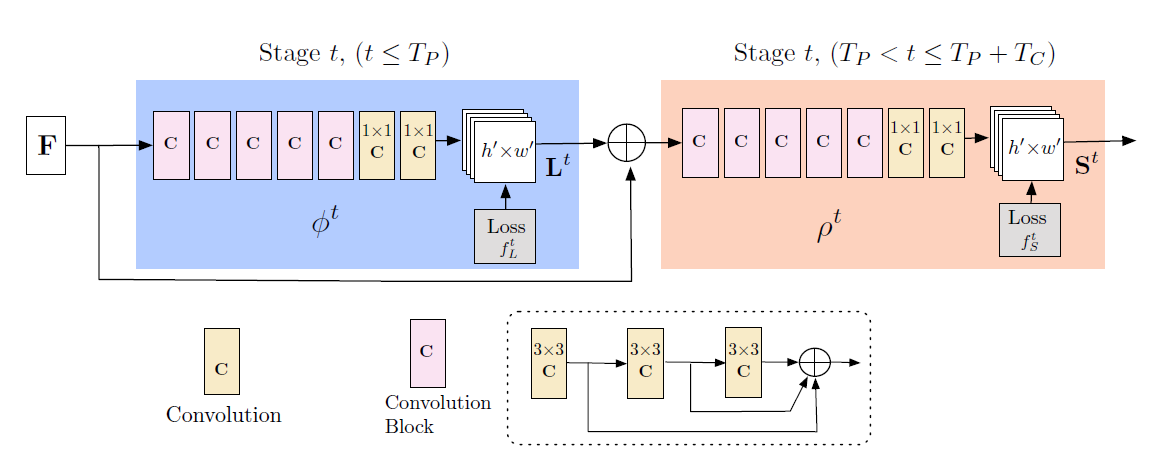
\includegraphics[width=\textwidth]{algoritme_architectuur}
	\end{figure}
\end{frame}

\begin{frame}
\frametitle{Voorbeeld van \textit{heatmap} en \textit{part affinity field}}
\begin{figure}
	\centering
	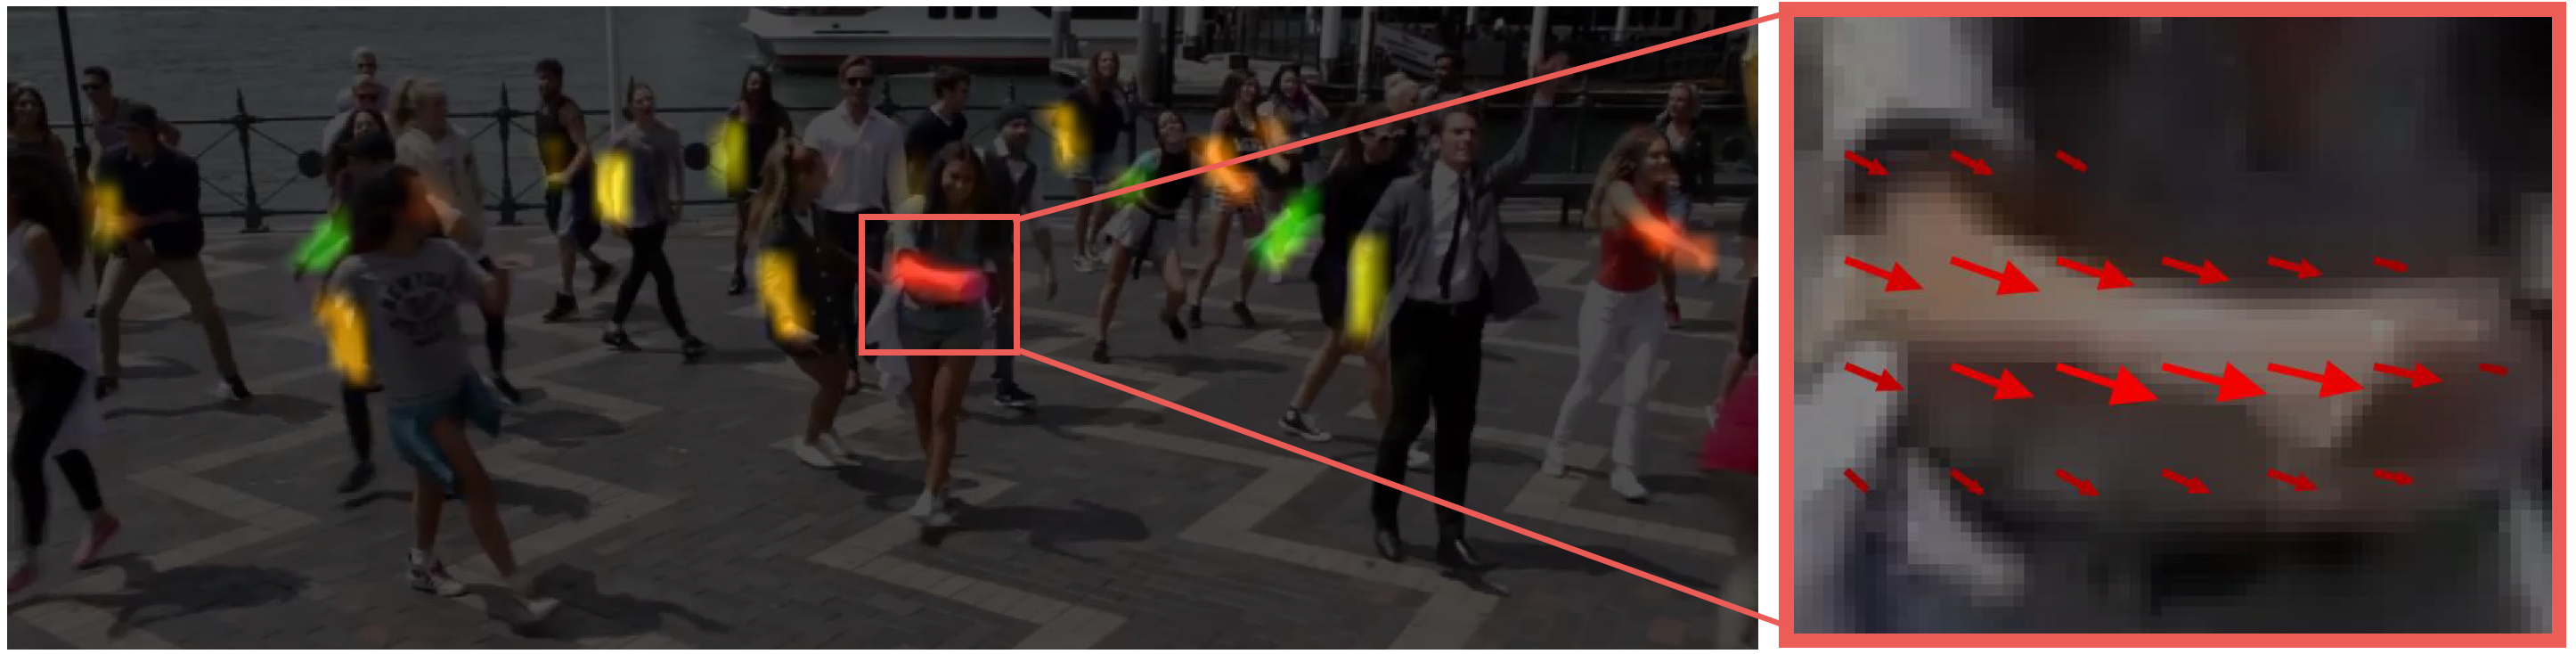
\includegraphics[width=\textwidth]{PAF}
\end{figure}
\end{frame}
\begin{frame}
\frametitle{Voorbeeld van \textit{heatmap} en \textit{part affinity field}}
	\begin{figure}
		\centering
		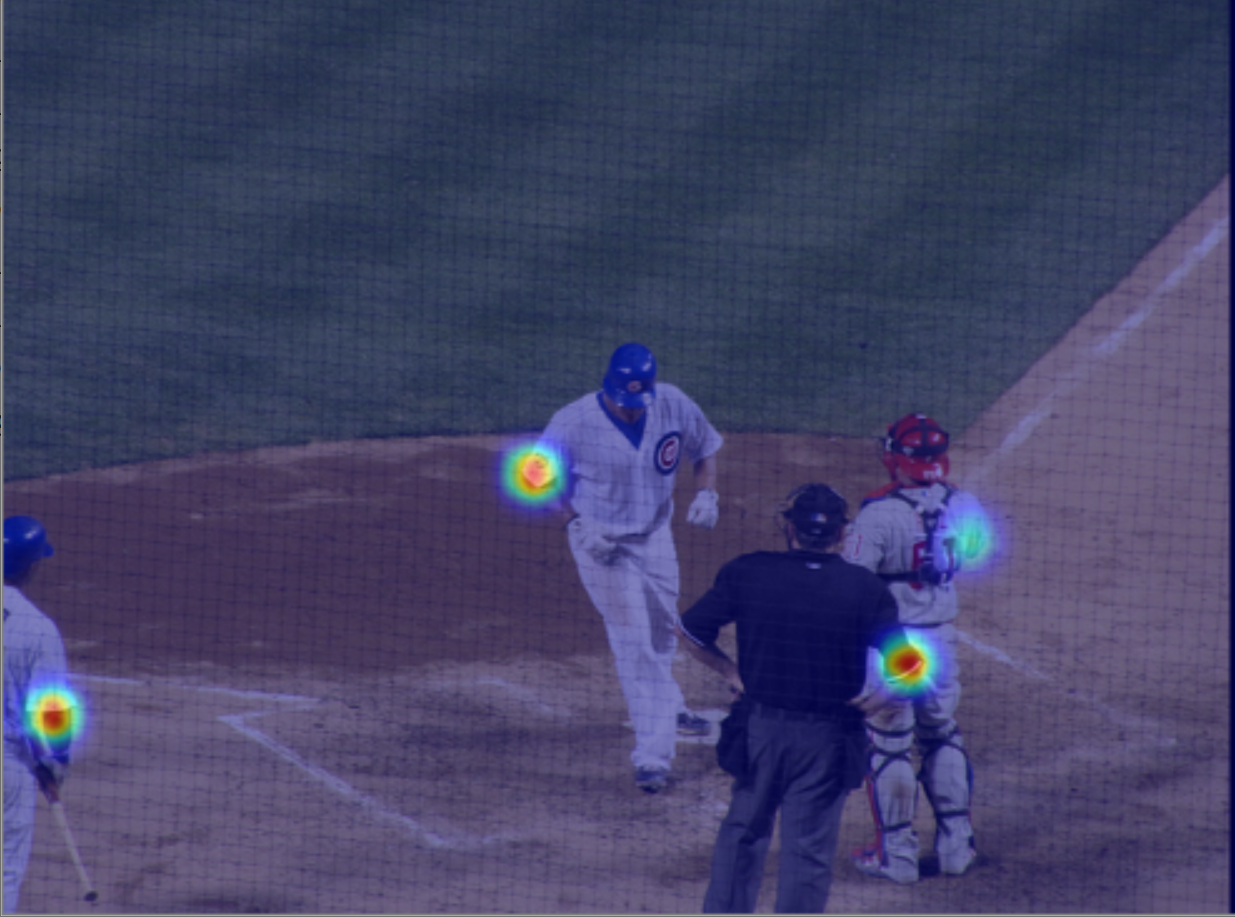
\includegraphics[width=0.8\textwidth]{heatmap_1}
	\end{figure}
\end{frame}



\section{Toepassing 1: Opvolgen van revalidatie na schouderoperatie}

\begin{frame}
\frametitle{Bepalen van de hoek tussen arm en borst}
\begin{itemize}
	\item hoek tussen [32] en [21] of [15] en [56]
	\item m.b.v. cosinusregel via coördinaten
\end{itemize}
\begin{figure}
	\centering
	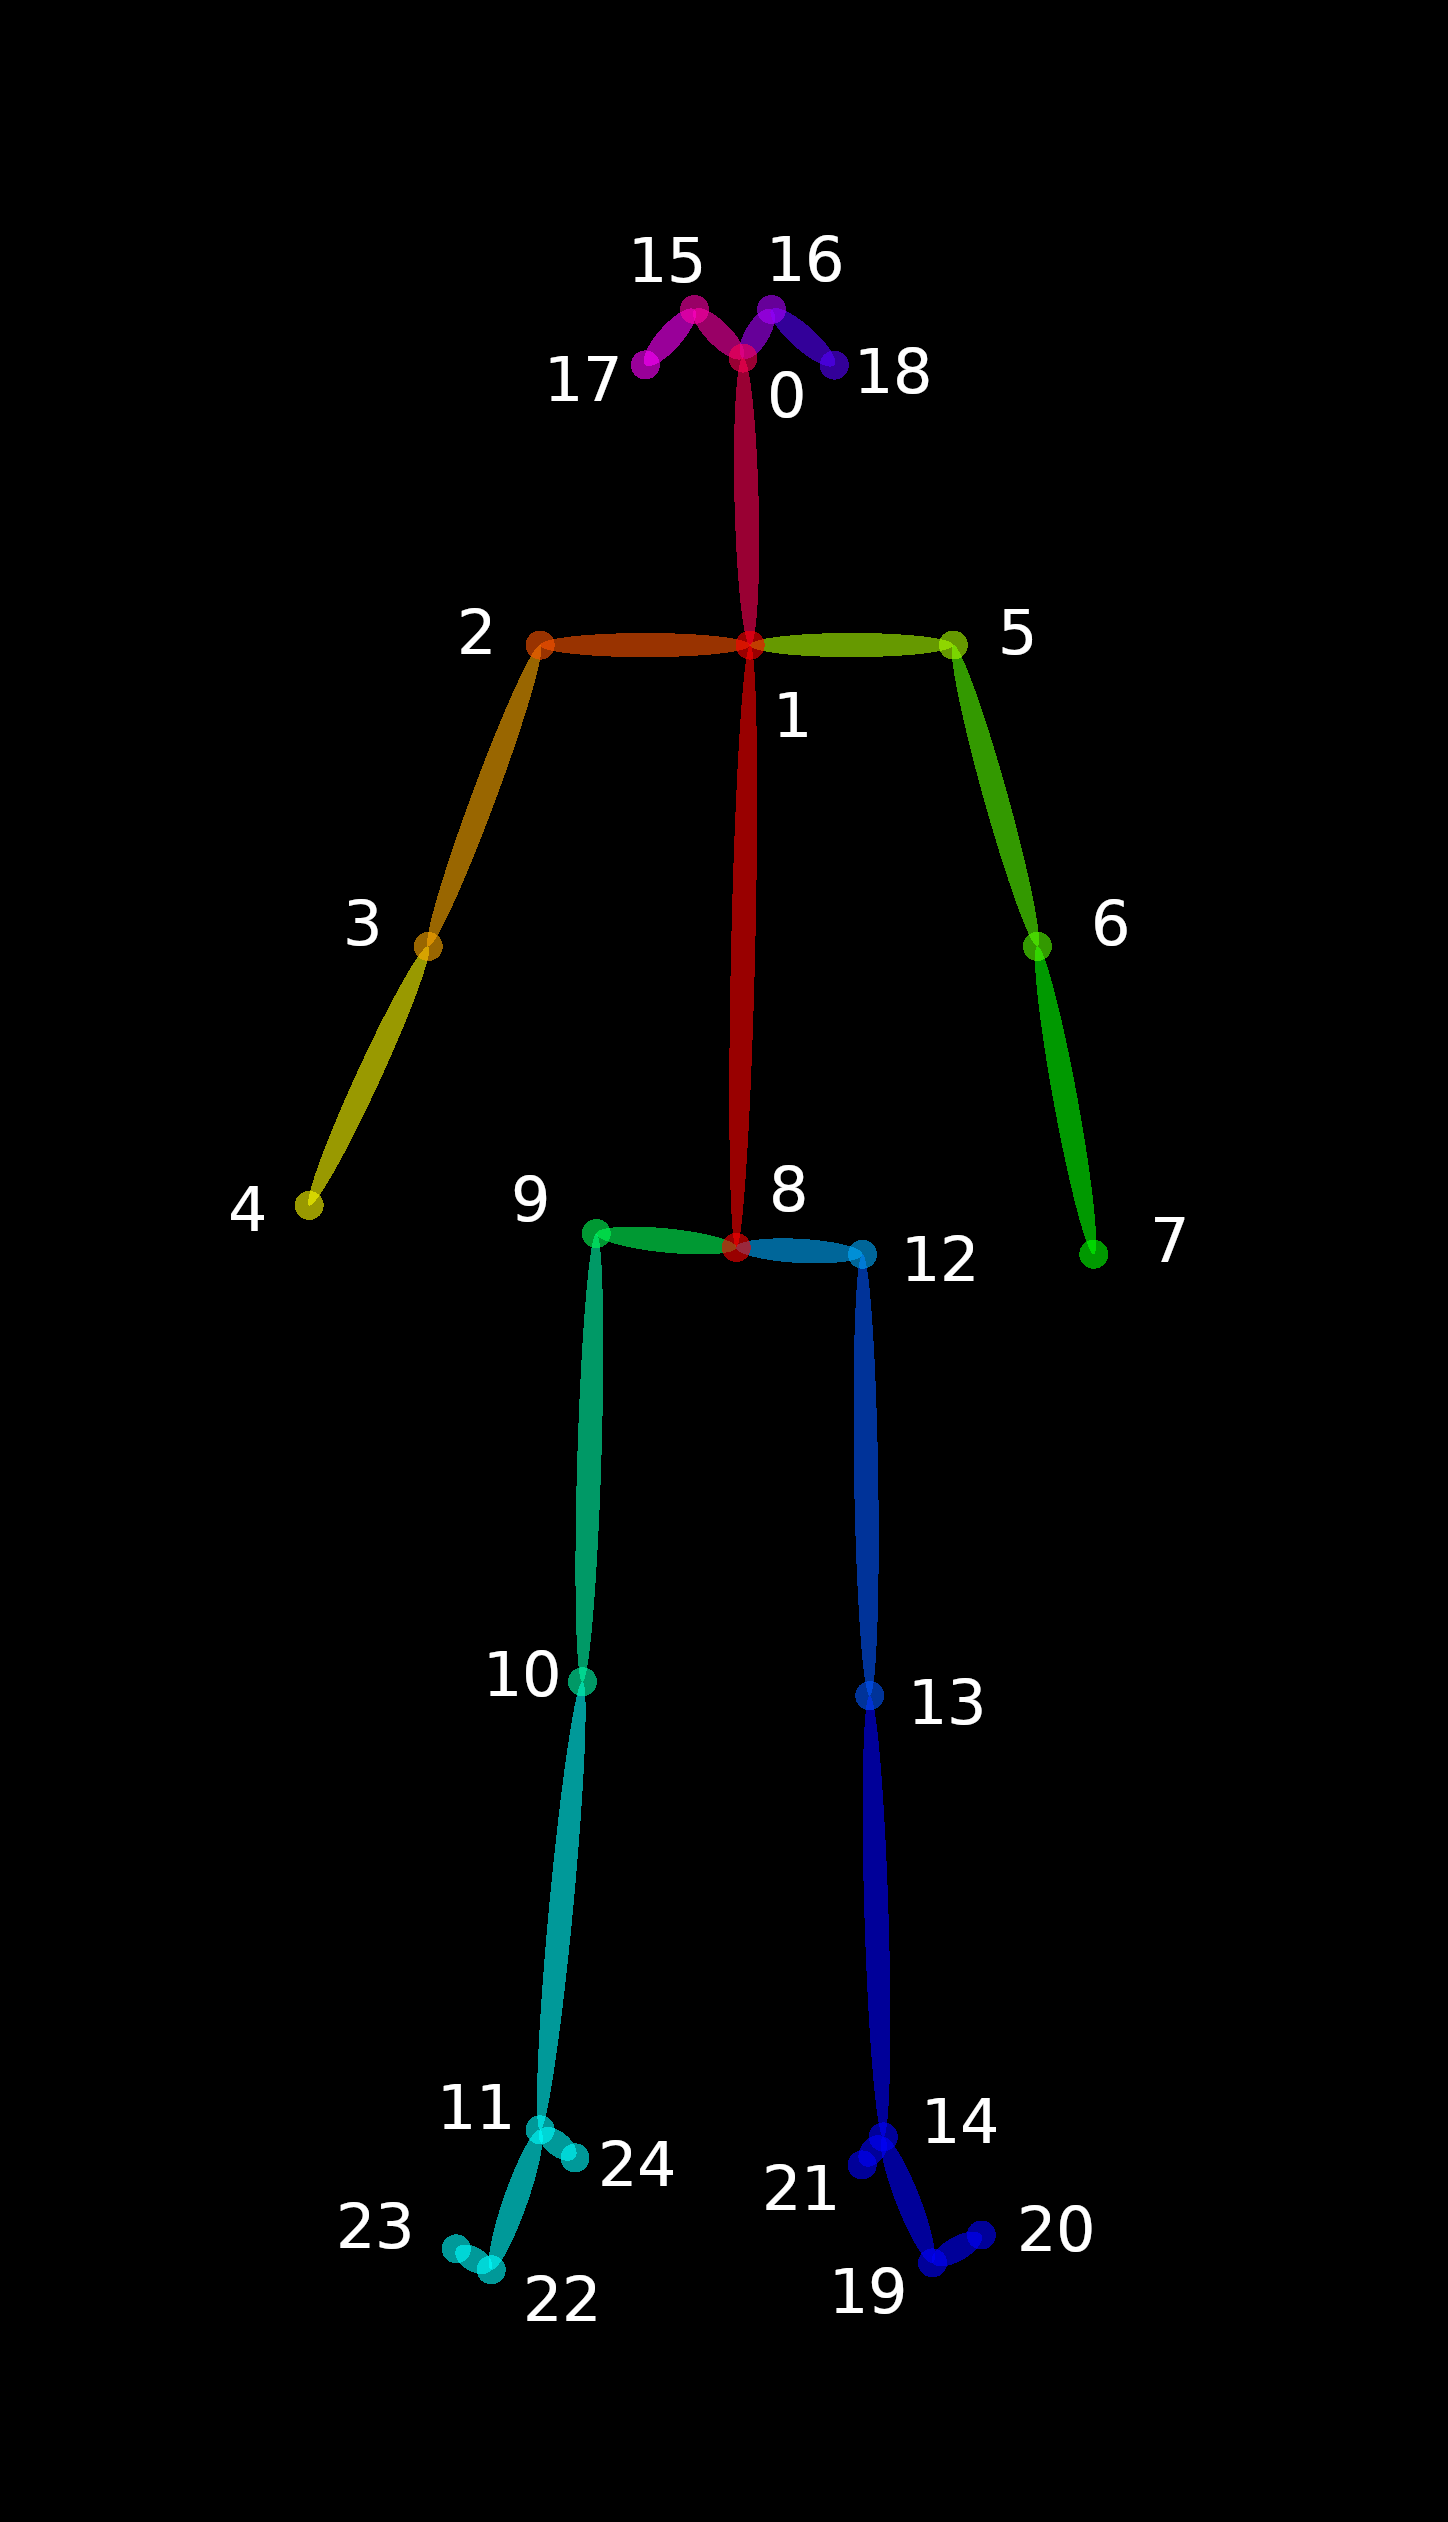
\includegraphics[width= .3\textwidth]{HPE_skelet}
\end{figure}
\end{frame}

\begin{frame}
\frametitle{Resultaten en conclusies}
\begin{itemize}
	\item foto recht nemen (Openpose werkt in 2D)
	\item telkens vanuit zelfde positie om revalidatie te evalueren
\end{itemize}
\begin{figure}
	\centering
	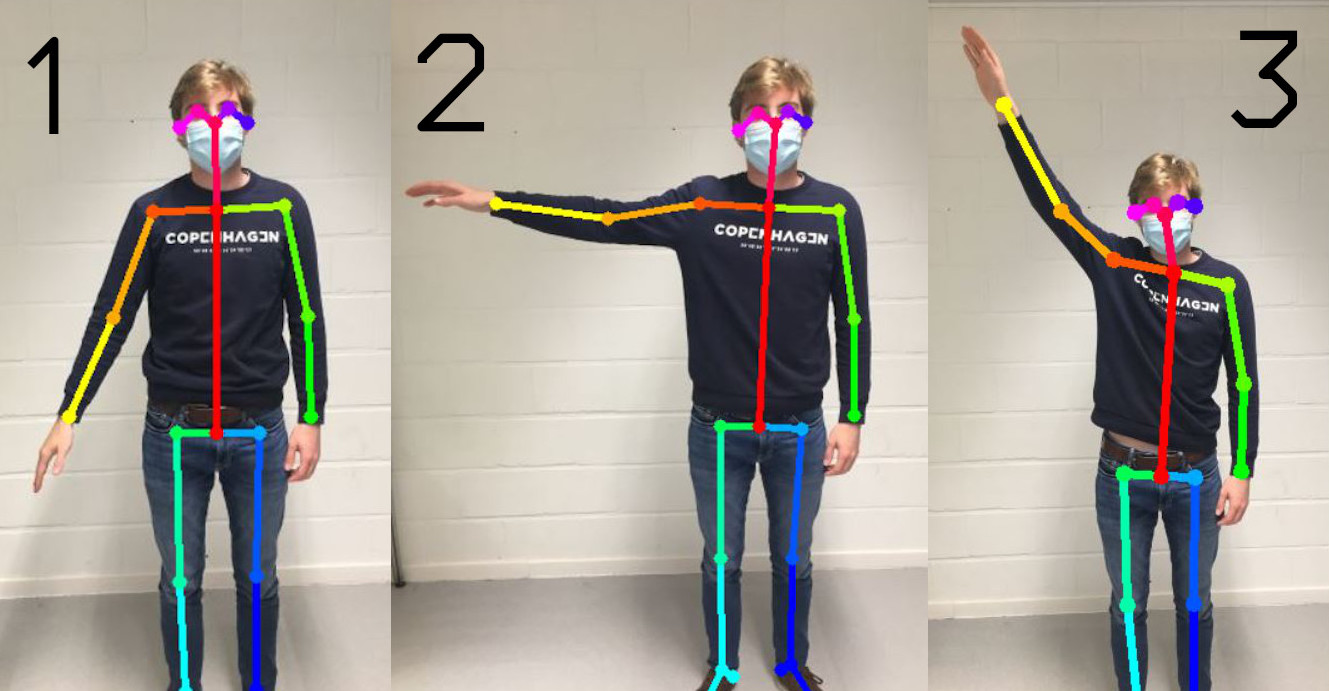
\includegraphics[width= \textwidth]{samen}
\end{figure}
\end{frame}



\section{Toepassing 2: Fietspositie bepalen}

\begin{frame}
	\frametitle{Wat is een bikefit?}
	\begin{itemize}
		\item analyseren van de positie op de fiets
		\item eventuele aanpassingen voorstellen obv analyse
		\item doel: blessurepreventie, aerodynamica en groter vermogen
	\end{itemize}
\begin{figure}
	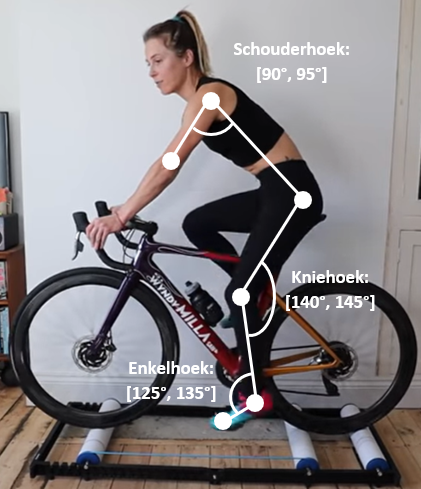
\includegraphics[width= .4\textwidth]{bikefit_hoeken_foto}
\end{figure}
\end{frame}

\begin{frame}
	\frametitle{Algoritme voor het wijzigen van de zadelhoogte}
	\begin{itemize}
		\item vooral zadelhoogte beïnvloedt kniehoek
		\item kniehoek moet tussen 140° en 145°
		\item pixels $\rightarrow$ \si{cm}
	\end{itemize}
	\begin{figure}
		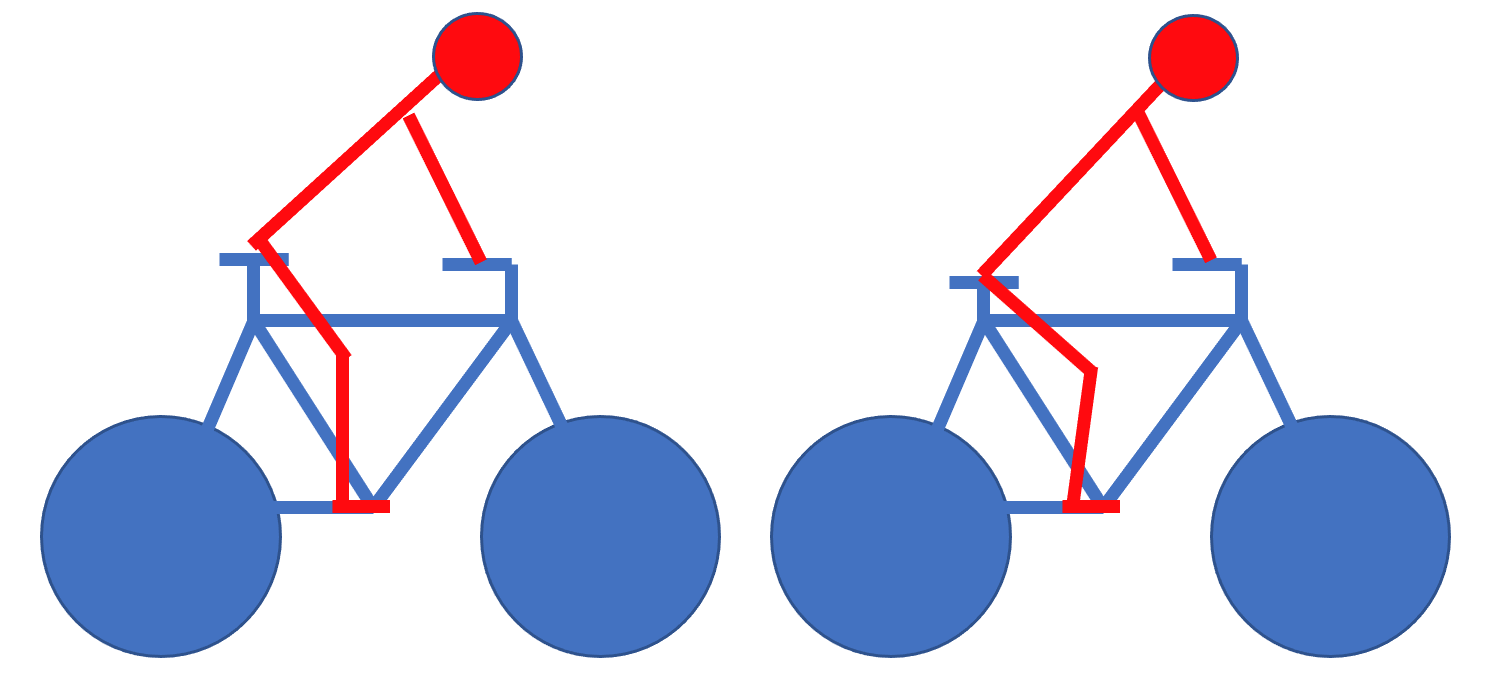
\includegraphics[width= \textwidth]{zadel.png}
	\end{figure}
\end{frame}

\begin{frame}
	\frametitle{Algoritme voor het wijzigen van de stuurpenlengte}
	\begin{itemize}
		\item vooral stuurpenlengte beïnvloedt schouderhoek
		\item bijna geen verandering aan de knie
		\item beschikbaar in lengte van 40 tot 140 \si{mm}
	\end{itemize}
	\begin{figure}
		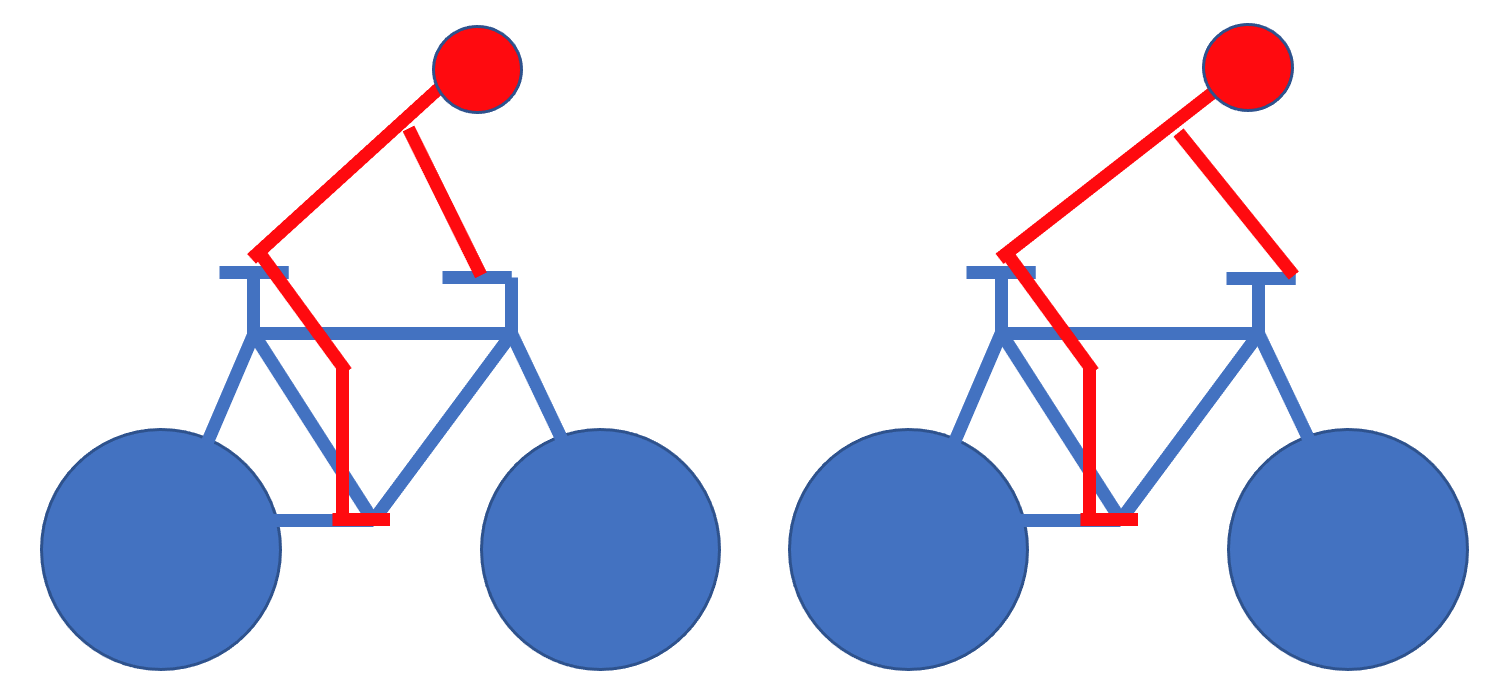
\includegraphics[width= \textwidth]{stuur.png}
	\end{figure}
\end{frame}

\begin{frame}
	\frametitle{Factoren die invloed hebben op de uitkomst}
	\begin{itemize}
		\item invloed van de resolutie
	\end{itemize}
	\begin{figure}
		\begin{minipage}[b]{.5\linewidth}
			\centering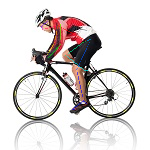
\includegraphics[width= \textwidth]{150x150}
			\subcaption{150x150}\label{fig:1a}
		\end{minipage}%
		\begin{minipage}[b]{.5\linewidth}
			\centering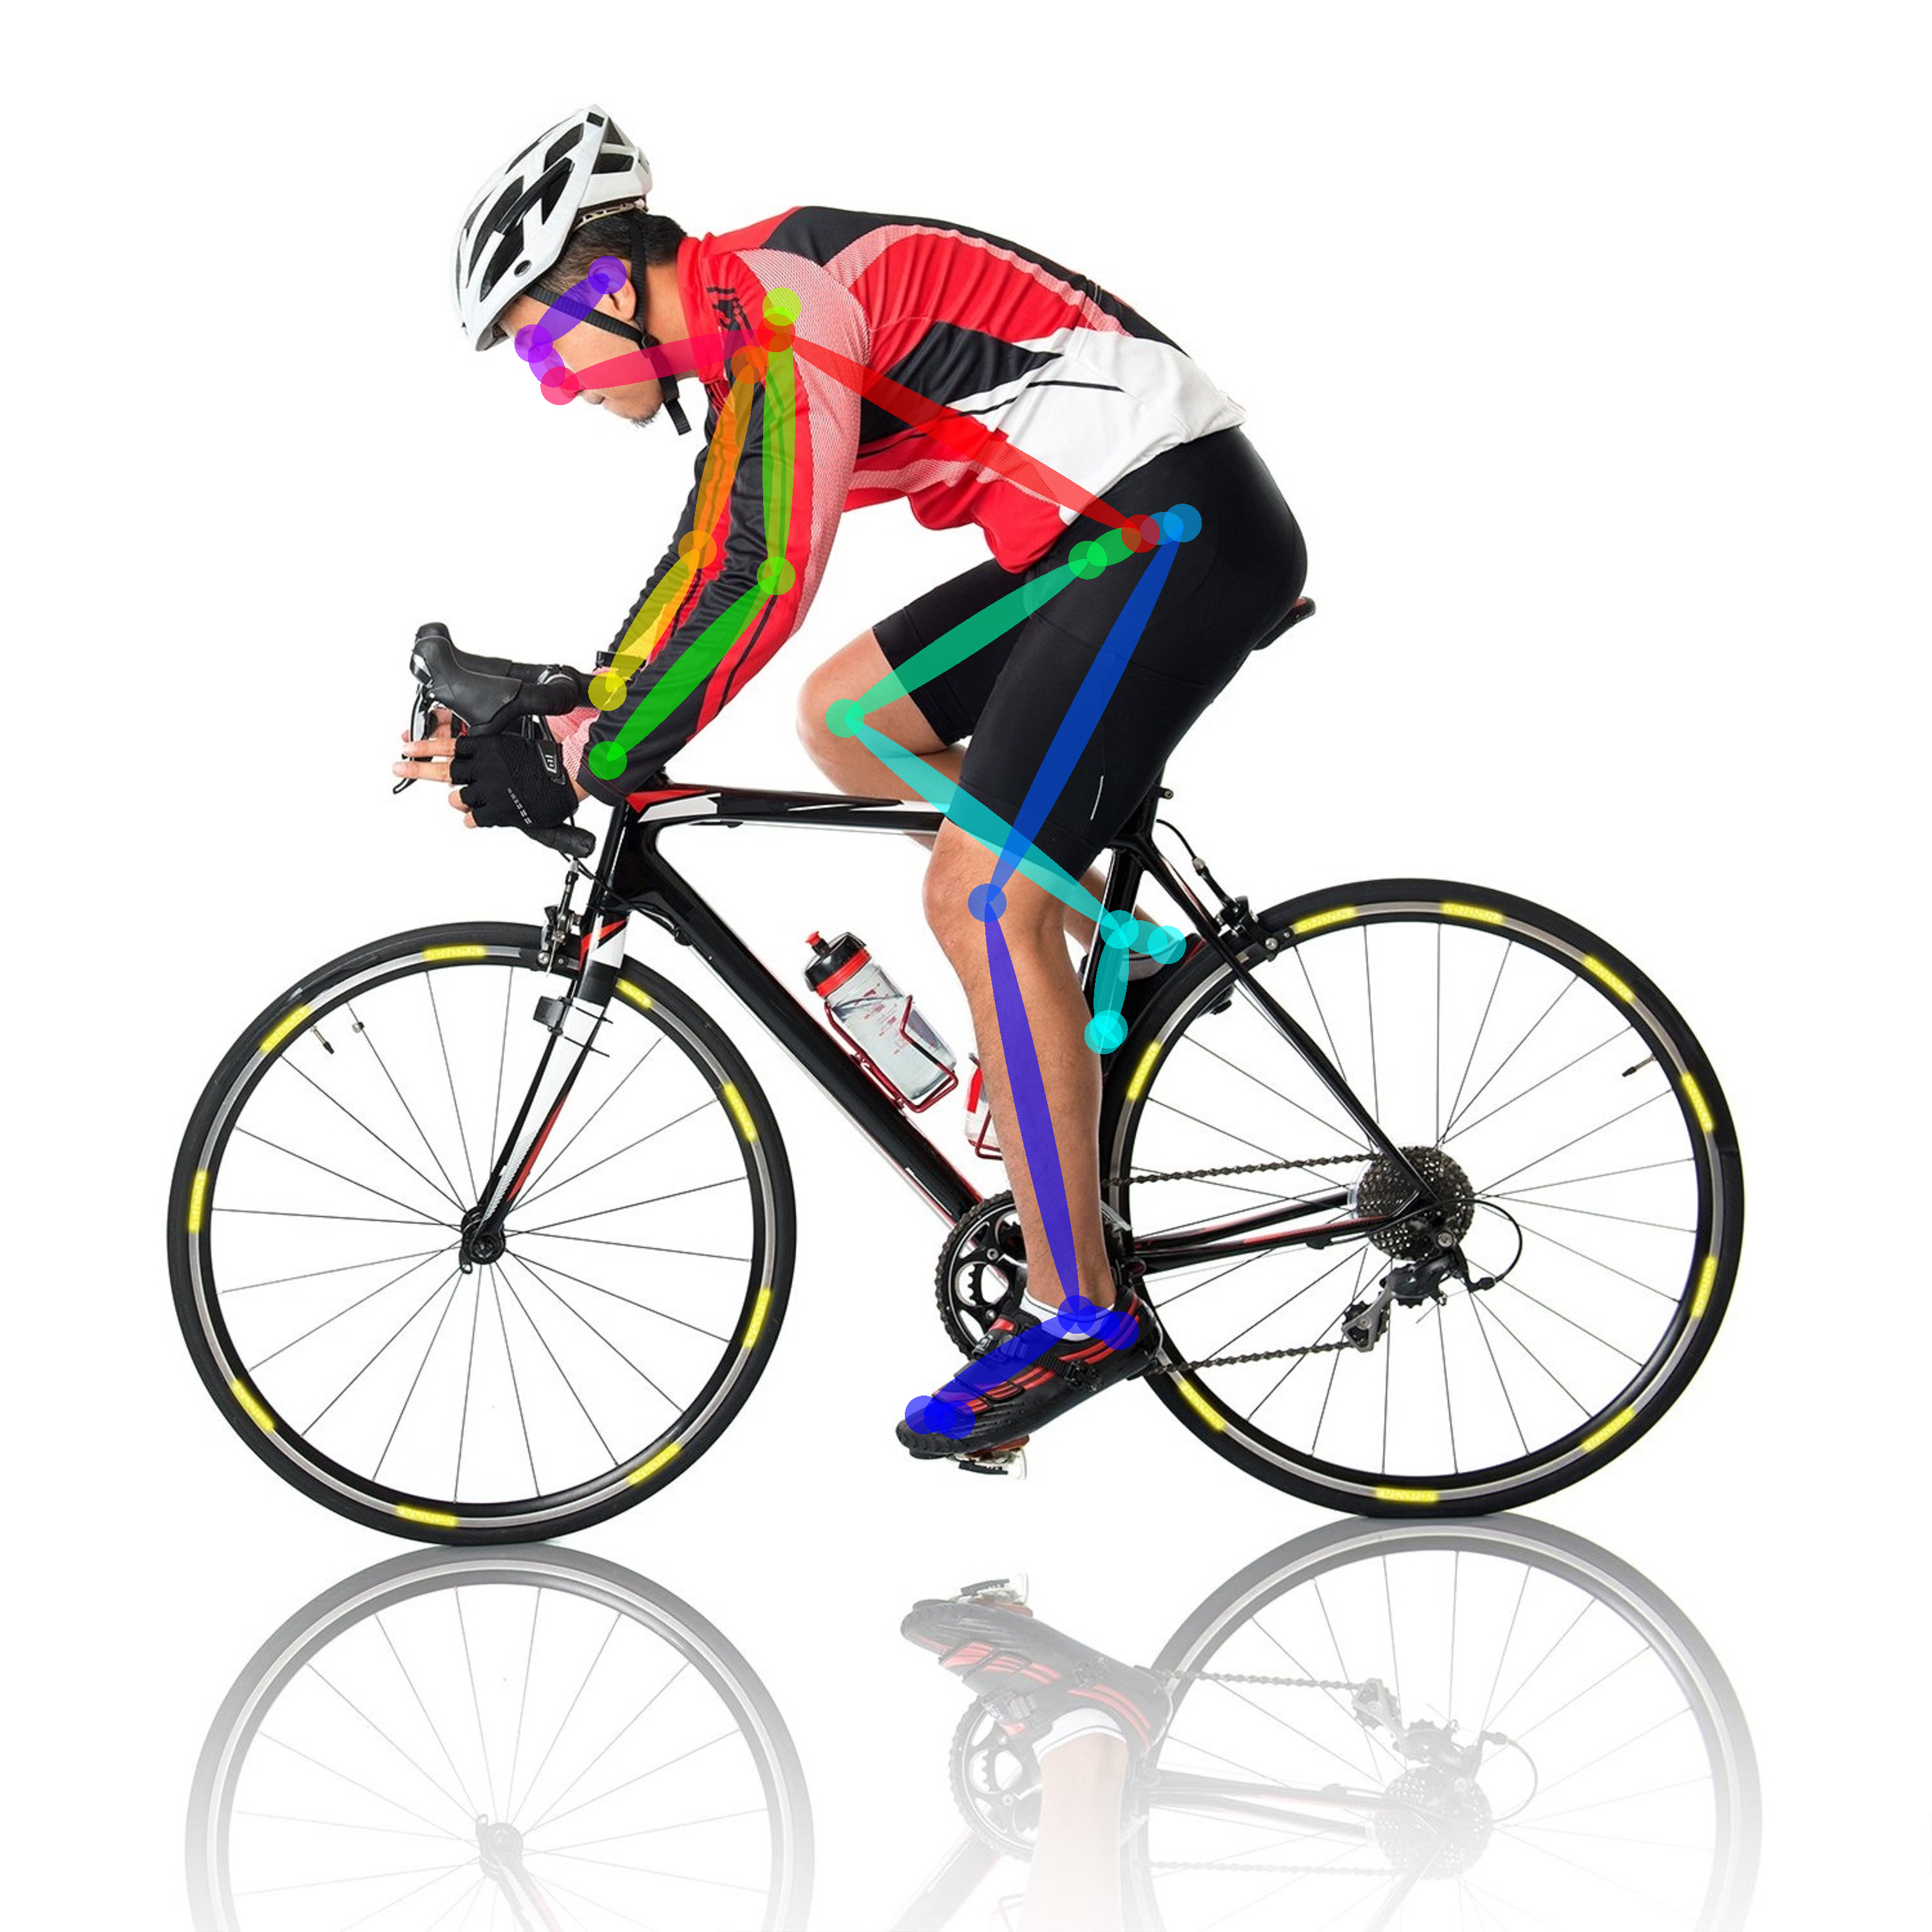
\includegraphics[width= \textwidth]{1500x1500}
			\subcaption{1500x1500}\label{fig:1b}
		\end{minipage}
		%\caption{A figure}\label{fig:1}
	\end{figure}
\end{frame}

\begin{frame}
	\frametitle{Factoren die invloed hebben op de uitkomst}
	\begin{itemize}
		\item fouten op omzetting van pixels naar \si{cm}
		\item pose is slechts een schatting van Openpose
	\end{itemize}
	\begin{figure}
		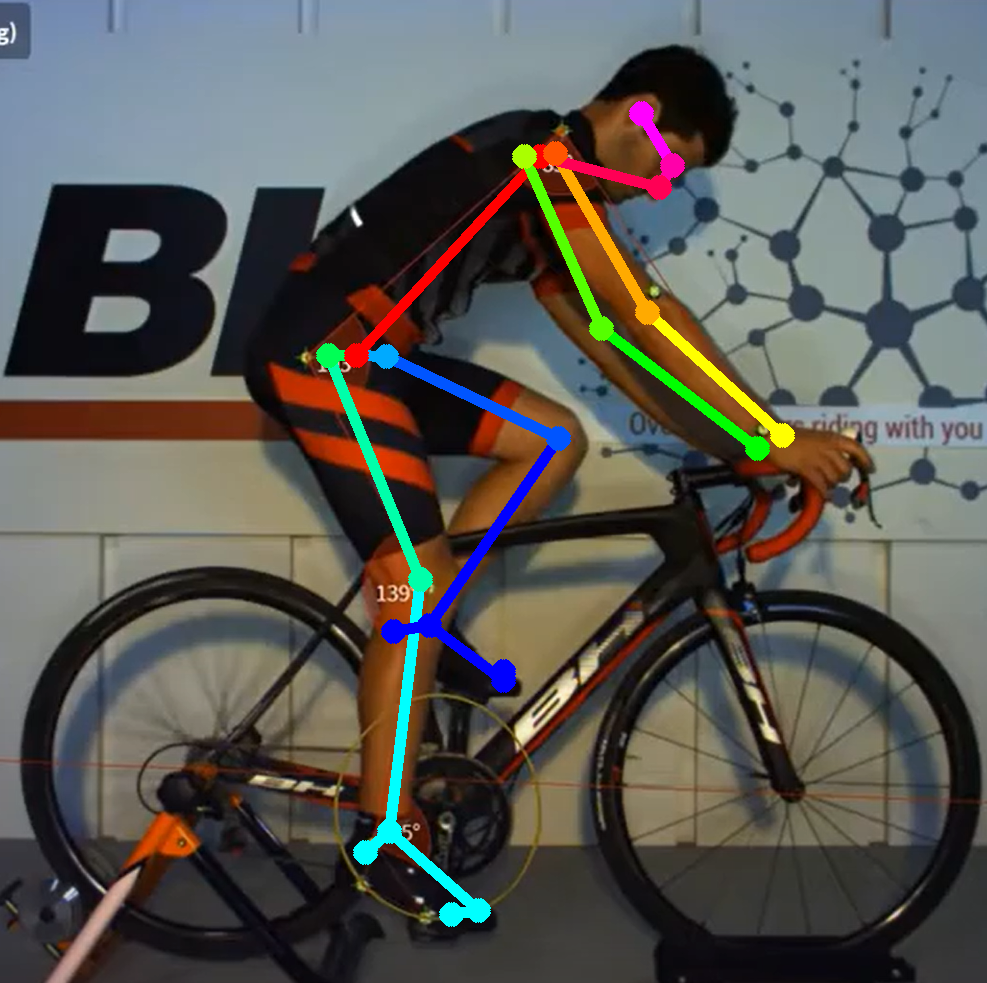
\includegraphics[width= .55\textwidth]{prof_bikefit}
	\end{figure}
\end{frame}

\begin{frame}
\frametitle{Conclusie}

\begin{center}
	Bikefitting heeft nood aan nauwkeurigheid\\
	$\updownarrow$ \\
	Openpose maakt slechts schatting
\end{center}


\end{frame}

\section{Toepassing 3: Correct uitvoeren van fitnessoefeningen}

\begin{frame}
	\frametitle{Richtlijnen voor een goeie squat}
	1. Knie boven de tenen
	\begin{figure}
		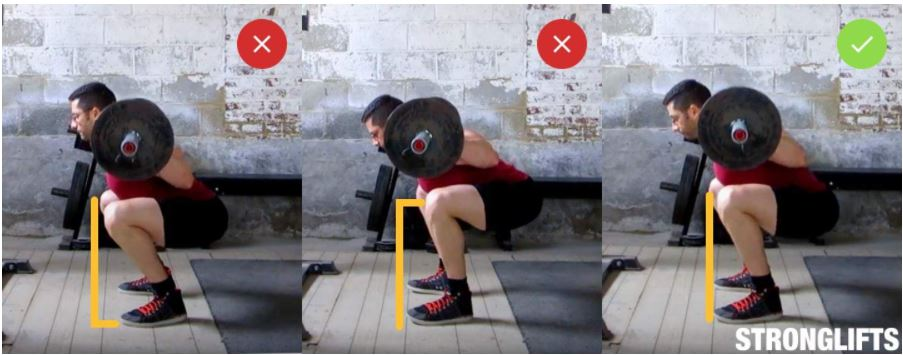
\includegraphics[width= \textwidth]{squat_knie}
	\end{figure}
\end{frame}

\begin{frame}
\frametitle{Richtlijnen voor een goeie squat}
2. Heup op dezelfde hoogte als knie
\begin{figure}
	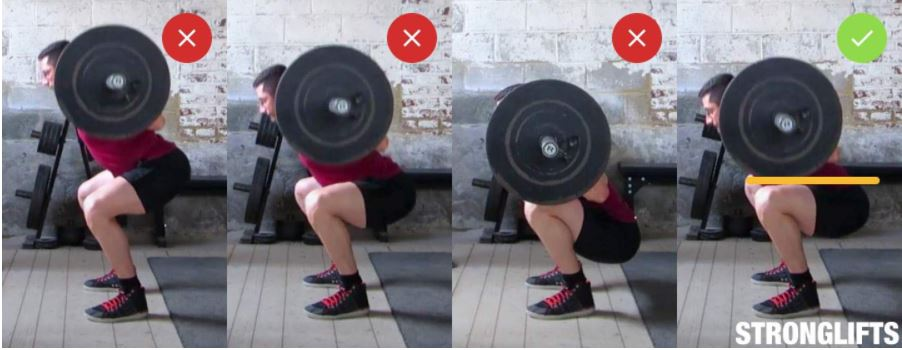
\includegraphics[width= \textwidth]{squat_heup}
\end{figure}
\end{frame}

\begin{frame}
	\frametitle{invloed van camerapositie}
	\begin{itemize}
		\item concreet antwoord vinden
		\item systematische aanpak
		\item testen door het varieren van:\begin{enumerate}
			\item afstand
			\item hoogte
			\item hoek
		\end{enumerate}
	\end{itemize}
\end{frame}

\begin{frame}
	\frametitle{invloed van camerapositie}
	De cameraopstelling
	\begin{figure}
		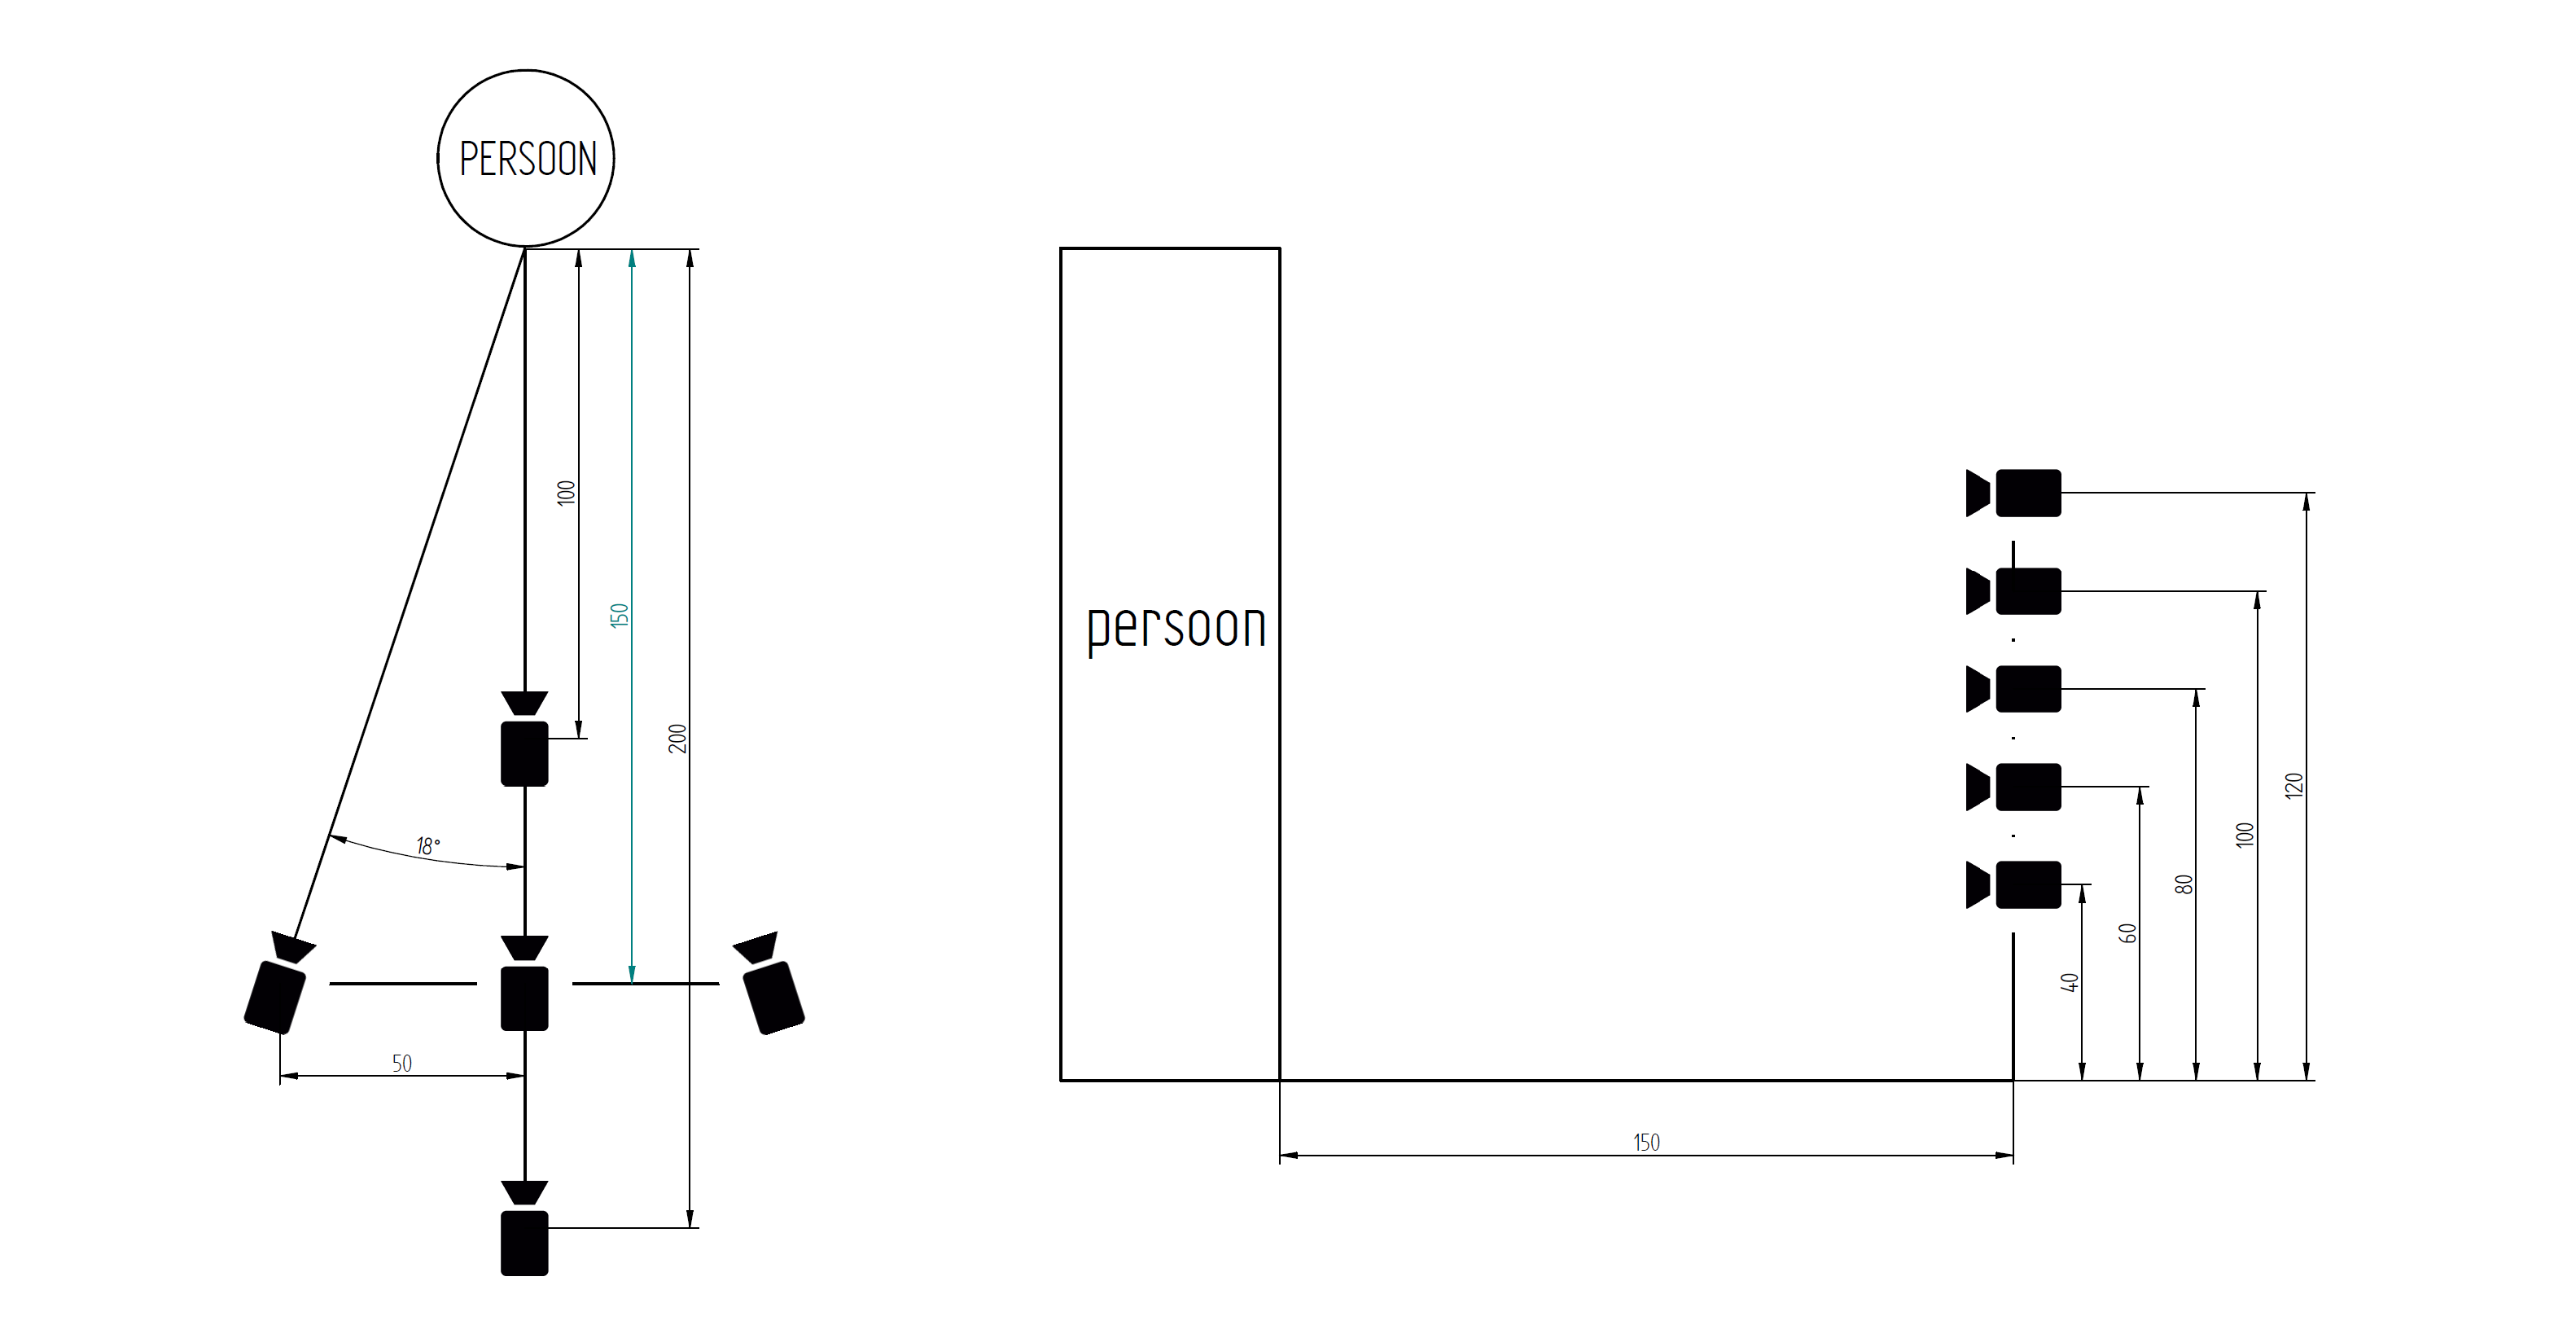
\includegraphics[width= \textwidth]{cameraopstelling}
	\end{figure}
\end{frame}

\section{Besluit}

\begin{frame}
\frametitle{Besluit}
\begin{itemize}
	\item niet geschikt voor medische toepassingen
	\item wel voor minder precieze doeleinden
	% Minder relevant maar ik wil dit er toch graag eens bij vermelden
	\item bijzonder moeilijke installatie
\end{itemize}
\end{frame}

\section*{Einde}
\begin{frame}
\frametitle{Einde}
\begin{center}
	Bedankt voor het luisteren\\
	Zijn er nog vragen?
\end{center}
\end{frame}
\end{document}
